\documentclass[11pt]{article}
\usepackage[margin=1in]{geometry}
\usepackage{amsmath,amssymb,booktabs}
\usepackage{graphicx}
\usepackage{hyperref}
\usepackage{xspace}

\newcommand{\E}{\mathbb{E}}
\newcommand{\T}{\mathbb{T}}
\newcommand{\uu}{\mathbf{u}}
\newcommand{\kk}{\mathbf{k}}
\newcommand{\pp}{\mathbf{p}}
\newcommand{\qq}{\mathbf{q}}
\newcommand{\xii}{\boldsymbol{\xi}}
\newcommand{\code}[1]{\texttt{#1}}
\newcommand{\SO}{\code{scalar\_only}\xspace}
\newcommand{\kin}{\code{kinematic}\xspace}
\newcommand{\STS}{RKL2 super-time-stepping\xspace}

\title{Prescribed-Velocity Scalar Mixing in AthenaK:\\
A Master Note on the Problem Statement, Spectral Roughness,\\
Velocity Construction, STS Diffusion, and Verification}
\author{}
\date{\today}

\begin{document}
\maketitle

\begin{abstract}
This document consolidates the scalar-mixing TeX notes in \code{./docs} into a single narrative. The organizing logic is the numerical problem itself. We begin with the passive-scalar question that motivates the calculations: whether a frozen, divergence-free, rough velocity field can sustain finite-time scalar dissipation as the diffusivity tends to zero, and how that transition depends on the geometry of the advecting field. We then translate between the two roughness languages used across the notes: the shell-integrated velocity spectrum $E_u(k)\propto k^{-\zeta}$ and the regularity index $\alpha$. That translation clarifies why $\alpha=(\zeta-1)/2$ is a classical H\"older exponent only when $1<\zeta<3$, while the regime $\alpha\le 0$ must be interpreted distributionally and approached numerically through ultraviolet-truncated approximations. With that dictionary in place, we document the four implemented solenoidal velocity generators in AthenaK: 2D projection, 2D stream function, 3D projection, and 3D Clebsch stream initialization. We then summarize the dedicated velocity-initialization tests and the independent scalar advection--diffusion verification problem, now including the \STS path used for parabolic scalar diffusion. The result is a single reference that starts from the scientific question, moves through the spectral and algorithmic setup, and ends with the tests that justify using the implementation for scalar-mixing studies.
\end{abstract}

\section{Problem Statement}
The broad problem is to understand passive-scalar mixing by a prescribed rough flow. Let $\theta=\theta(x,t)$ solve
\begin{equation}
\partial_t \theta + \uu\cdot\nabla \theta = D\Delta\theta,
\qquad
\nabla\cdot\uu = 0,
\label{eq:scalar}
\end{equation}
on the periodic box $\T^d$ with $d\in\{2,3\}$, scalar diffusivity $D>0$, and fixed initial data $\theta_0$. In the AthenaK scalar-mixing problems the velocity field is autonomous: one random realization of $\uu(x)$ is generated at $t=0$ and then held fixed while the scalar evolves.

The principal observable is the finite-time integrated scalar dissipation
\begin{equation}
\chi_D(T) = D\int_0^T\int_{\T^d} |\nabla\theta(x,t)|^2\,dx\,dt.
\label{eq:chi}
\end{equation}
The time horizon $T$ must remain finite. Because the velocity is frozen, the scalar eventually relaxes to its spatial mean and the long-time problem becomes trivial. The interesting question is therefore a finite-time one: over one to a few advective times, does the scalar continue to dissipate an order-unity amount of variance as $D\to 0$, or does the dissipation collapse?

This immediately leads to the anomalous-dissipation question. For a given velocity ensemble, does one observe
\begin{equation}
\liminf_{D\to 0}\E[\chi_D(T)]>0
\label{eq:anomalous}
\end{equation}
for finite $T$ of advective order, or instead $\E[\chi_D(T)]\to 0$? A second question is whether the scalar itself develops a predictable regularity exponent $\beta$, for example through second-order increments
\begin{equation}
\E|\theta(x+h,t)-\theta(x,t)|^2 \sim |h|^{2\beta},
\label{eq:theta-structure}
\end{equation}
and whether this exponent is related to the velocity roughness by the Yaglom-type relation
\begin{equation}
\alpha + 2\beta = 1.
\label{eq:yaglom}
\end{equation}
The practical objective is to identify a roughness threshold separating weak-mixing from anomalous-dissipation behavior, and then determine whether that threshold depends only on the nominal roughness of the velocity field or also on how incompressibility is realized.

AthenaK now supports four prescribed velocity generators for this purpose:
\begin{enumerate}
\item 2D projection,
\item 2D stream function, $\uu=\nabla^\perp\psi$,
\item 3D projection,
\item 3D Clebsch stream, $\uu=\nabla\phi_1\times\nabla\phi_2$.
\end{enumerate}
The scientific comparison is therefore not merely between dimensions. It is also between linear projection-based solenoidal fields and stream-based constructions that impose additional latent structure through one or two scalar potentials.

\section{From H\"older Exponents to Power Spectra}
The next step is to translate between the two roughness languages used across the notes. In physical language one prescribes a shell-integrated velocity spectrum
\begin{equation}
E_u(k)\propto k^{-\zeta},
\label{eq:eu}
\end{equation}
where $k$ denotes isotropic shell index or wave-number magnitude. In mathematical language one would like to speak about the regularity of the field.

For an isotropic random field with Fourier coefficients
\begin{equation}
\widehat{u}(\kk)=\sigma(|\kk|)g_\kk,
\qquad
\E|g_\kk|^2=1,
\end{equation}
the shell spectrum and coefficient variance are related by shell counting:
\begin{equation}
E_u(k)\sim k^{d-1}\sigma(k)^2.
\label{eq:shell-count}
\end{equation}
Therefore, if $E_u(k)\sim k^{-\zeta}$, then
\begin{equation}
\sigma(k)^2 \sim k^{-(\zeta+d-1)},
\qquad
\sigma(k)\sim k^{-(\zeta+d-1)/2}.
\label{eq:sigma-law}
\end{equation}
This is the basic bridge between the spectrum seen by a physicist and the mode-by-mode variance seen by a mathematician.

There is a second bridge, from the spectrum to regularity. When
\begin{equation}
1<\zeta<3,
\label{eq:zeta-window}
\end{equation}
the second-order increment law is well behaved:
\begin{equation}
\E|\uu(x+h)-\uu(x)|^2 \sim |h|^{\zeta-1}.
\end{equation}
In this regime one may identify the classical H\"older exponent
\begin{equation}
\alpha = \frac{\zeta-1}{2},
\qquad
0<\alpha<1.
\label{eq:alpha-zeta}
\end{equation}
This is the range in which the usual statement ``Kolmogorov $-5/3$ corresponds to $\alpha=1/3$'' is literally a pointwise regularity statement.

The important caveat is that Equation~(\ref{eq:alpha-zeta}) continues to be a useful roughness dictionary even when $\zeta\le 1$, but it must then be interpreted differently. If
\begin{equation}
-1\le \zeta \le 1,
\qquad
-1\le \alpha \le 0,
\end{equation}
the continuum field is too rough for a classical pointwise H\"older interpretation. In that regime $\alpha$ should instead be read as a negative regularity index, for example in a Sobolev or H\"older--Besov sense. One convenient way to see the same threshold is through the shell sum
\begin{equation}
\sum_k k^{2s}E_u(k),
\end{equation}
whose ultraviolet convergence becomes marginal at $s=\alpha=(\zeta-1)/2$.

This distinction matters numerically. At any fixed cutoff AthenaK generates a finite trigonometric polynomial, so every realized field is smooth. The regime $\alpha\le 0$ is therefore not produced as a literal negative-regularity field at fixed resolution. It is explored through a sequence of ultraviolet-truncated approximations with increasing $k_{\max}$. In other words, the code controls $\zeta$ directly, while the continuum interpretation of $\alpha$ depends on how the cutoff is taken.

The same spectral translation also fixes the mode-variance laws for the latent fields used by the stream constructions. The summary relevant for AthenaK is given in Table~\ref{tab:variance-laws}.

\begin{table}[t]
\centering
\caption{Coefficient-variance laws corresponding to the target velocity spectrum $E_u(k)\propto k^{-\zeta}$.}
\label{tab:variance-laws}
\begin{tabular}{@{}lll@{}}
\toprule
Field & Complex-mode variance & Amplitude law \\
\midrule
2D velocity $\hat{\uu}(\kk)$
& $\E |\hat{\uu}(\kk)|^2 \propto |\kk|^{-(\zeta+1)}$
& $|\kk|^{-(\zeta+1)/2}$ \\
3D velocity $\hat{\uu}(\kk)$
& $\E |\hat{\uu}(\kk)|^2 \propto |\kk|^{-(\zeta+2)}$
& $|\kk|^{-(\zeta+2)/2}$ \\
2D stream $\hat{\psi}(\kk)$
& $\E |\hat{\psi}(\kk)|^2 \propto |\kk|^{-(\zeta+3)}$
& $|\kk|^{-(\zeta+3)/2}$ \\
3D Clebsch $\hat{\phi}_1,\hat{\phi}_2$
& no settled universal continuum law;
  AthenaK fits discrete shell powers
& multi-start numerical fit against the exact tensor \\
\bottomrule
\end{tabular}
\end{table}

\section{Velocity Field Setup}
The implementation then turns the target spectrum into a concrete divergence-free realization. Across all four generators, the user-facing control parameters are interpreted in terms of the \emph{velocity field}: the driving band is set by \code{turb\_nlow} and \code{turb\_nhigh}, the shell-integrated slope by \code{turb\_expo}, the final amplitude by \code{turb\_v\_rms}, and the retained-mode thinning by \code{turb\_k\_crit}.

\subsection{Common Spectral Framework}
AthenaK writes the initialized field as a real retained half-space series,
\begin{equation}
\uu(\mathbf{x}) =
\sum_{\mathbf{n}\in\mathcal{H}_{\rm kept}}
\left[\mathbf{a}_{\mathbf{n}}\cos(\kk_{\mathbf{n}}\cdot\mathbf{x})
- \mathbf{b}_{\mathbf{n}}\sin(\kk_{\mathbf{n}}\cdot\mathbf{x})\right],
\label{eq:halfspace}
\end{equation}
where $\mathcal{H}_{\rm kept}$ contains exactly one representative of each implicit complex-conjugate pair. This makes the initialized field real by construction while still allowing the generator to work mode by mode in Fourier space.

The kept catalog is built in two stages. First, the code enumerates all admissible half-space modes in the requested band. Second, it performs importance sampling above the user scale \code{turb\_k\_crit}. The acceptance probability is
\begin{equation}
p_{\rm acc}(k)=
\left\{
\begin{array}{ll}
1, & k<k_{\rm crit}, \\
(k_{\rm crit}/k)^2, & k\ge k_{\rm crit},
\end{array}
\right.
\end{equation}
and each retained mode is multiplied by $p_{\rm acc}^{-1/2}$ so that shell-integrated variances remain unbiased. After synthesis, AthenaK removes any residual mean flow and applies a uniform rescaling so that the final field matches the requested rms speed. The problem generator can also dump a reproducibility sidecar, \code{basename.turb\_init\_diag.json}, containing retained mode catalogs, coefficients, shell spectra, and latent stream fields.

\subsection{Two-Dimensional Generators}
In 2D projection mode the code draws Gaussian vector coefficients and then removes the component parallel to $\kk$. To recover the target shell spectrum, the velocity coefficient amplitude must scale as
\begin{equation}
|\uu_{\kk}| \propto k^{-(\zeta+1)/2}.
\label{eq:2d-proj}
\end{equation}
This is the direct spectral route: the stored coefficients are already velocity coefficients.

In 2D stream mode the code instead synthesizes
\begin{equation}
\psi(\mathbf{x}) = \sum_{\mathbf{n}\in\mathcal{H}_{\rm kept}}
\left[a^\psi_{\mathbf{n}}\cos(\kk_{\mathbf{n}}\cdot\mathbf{x})
- b^\psi_{\mathbf{n}}\sin(\kk_{\mathbf{n}}\cdot\mathbf{x})\right]
\end{equation}
and defines
\begin{equation}
\uu = (\partial_y\psi,\,-\partial_x\psi,\,0).
\label{eq:2d-stream}
\end{equation}
Because differentiation contributes one power of $k$, the stream-function coefficients must scale one power steeper:
\begin{equation}
|\psi_{\kk}| \propto k^{-(\zeta+3)/2}.
\label{eq:psi-law}
\end{equation}
The user still specifies the \emph{velocity} spectrum. AthenaK determines the compatible stream-function spectrum automatically.

\subsection{Three-Dimensional Generators}
The 3D projection construction is again linear. Random vector coefficients are drawn, projected perpendicular to $\kk$, and synthesized with amplitude law
\begin{equation}
|\uu_{\kk}| \propto k^{-(\zeta+2)/2},
\label{eq:3d-proj}
\end{equation}
which is the correct shell-count correction for three dimensions.

The 3D stream construction is qualitatively different. The initialized field is
\begin{equation}
\uu = \nabla\phi_1\times\nabla\phi_2.
\label{eq:clebsch}
\end{equation}
In Fourier space,
\begin{equation}
\hat{\uu}(\xii) =
-\sum_{\pp+\qq=\xii}
(\pp\times\qq)\,\hat{\phi}_1(\pp)\hat{\phi}_2(\qq).
\label{eq:clebsch-convolution}
\end{equation}
The velocity spectrum is therefore a quadratic functional of the two potentials.
The current AthenaK implementation no longer tries to solve an inverse shell-fit
problem for $\phi_1$ and $\phi_2$. Instead it mirrors the retained-mode
construction used in the companion notebook: the user specifies
\code{problem/turb\_velocity\_method=clebsch} together with a desired velocity
roughness parameter \code{problem/turb\_alpha}, AthenaK converts that to a
target shell slope for the scalar potentials,
\begin{equation}
s_\phi =
\begin{cases}
3 + 2\alpha, & \alpha \ge 0,\\
3 + \alpha, & \alpha < 0,
\end{cases}
\qquad
s_u = 2\alpha + 1,
\end{equation}
draws Gaussian scalar coefficients on the retained mode catalog, rescales each
retained shell so that $E_{\phi_1}(k)$ and $E_{\phi_2}(k)$ are exact
$k^{-s_\phi}$ laws on the accepted shell band, forms the retained Clebsch
velocity coefficients from Equation~(\ref{eq:clebsch-convolution}), and finally
normalizes the realized velocity field to zero mean and the requested rms
amplitude.

This means the latent scalar spectra are now simple, explicit auxiliary objects
rather than outputs of a separate optimizer. The user-facing caveat is equally
simple: because the initialized velocity is built on the retained mode catalog
and the Clebsch map is quadratic, the resulting velocity slope is only
approximate in practice, especially when \code{turb\_k\_crit} is small enough to
thin the high-$k$ catalog aggressively.

\section{Velocity Setup Tests}
The velocity generator is tested first, before any scalar problem is run on top of it. The reference campaign uses a common target slope $\zeta=5/3$, band $k\in[2,128]$, and unit rms speed. The 2D cases use $512^2$ with \code{turb\_k\_crit}=128. The 3D cases use $256^3$ with \code{turb\_k\_crit}=2.

Figure~\ref{fig:overview} gives the global comparison. All four initialized
fields are normalized to the requested rms speed and remain spectrally
divergence-free to roundoff-level accuracy. The two projection methods are
still the most direct route to a target velocity spectrum. The 3D Clebsch field
is now easier to interpret: the latent scalar spectra are exact retained-shell
power laws by construction, while the realized velocity spectrum follows the
requested slope only approximately because the Clebsch map is quadratic and the
3D retained catalog is importance-sampled.

\begin{figure}[t]
\centering
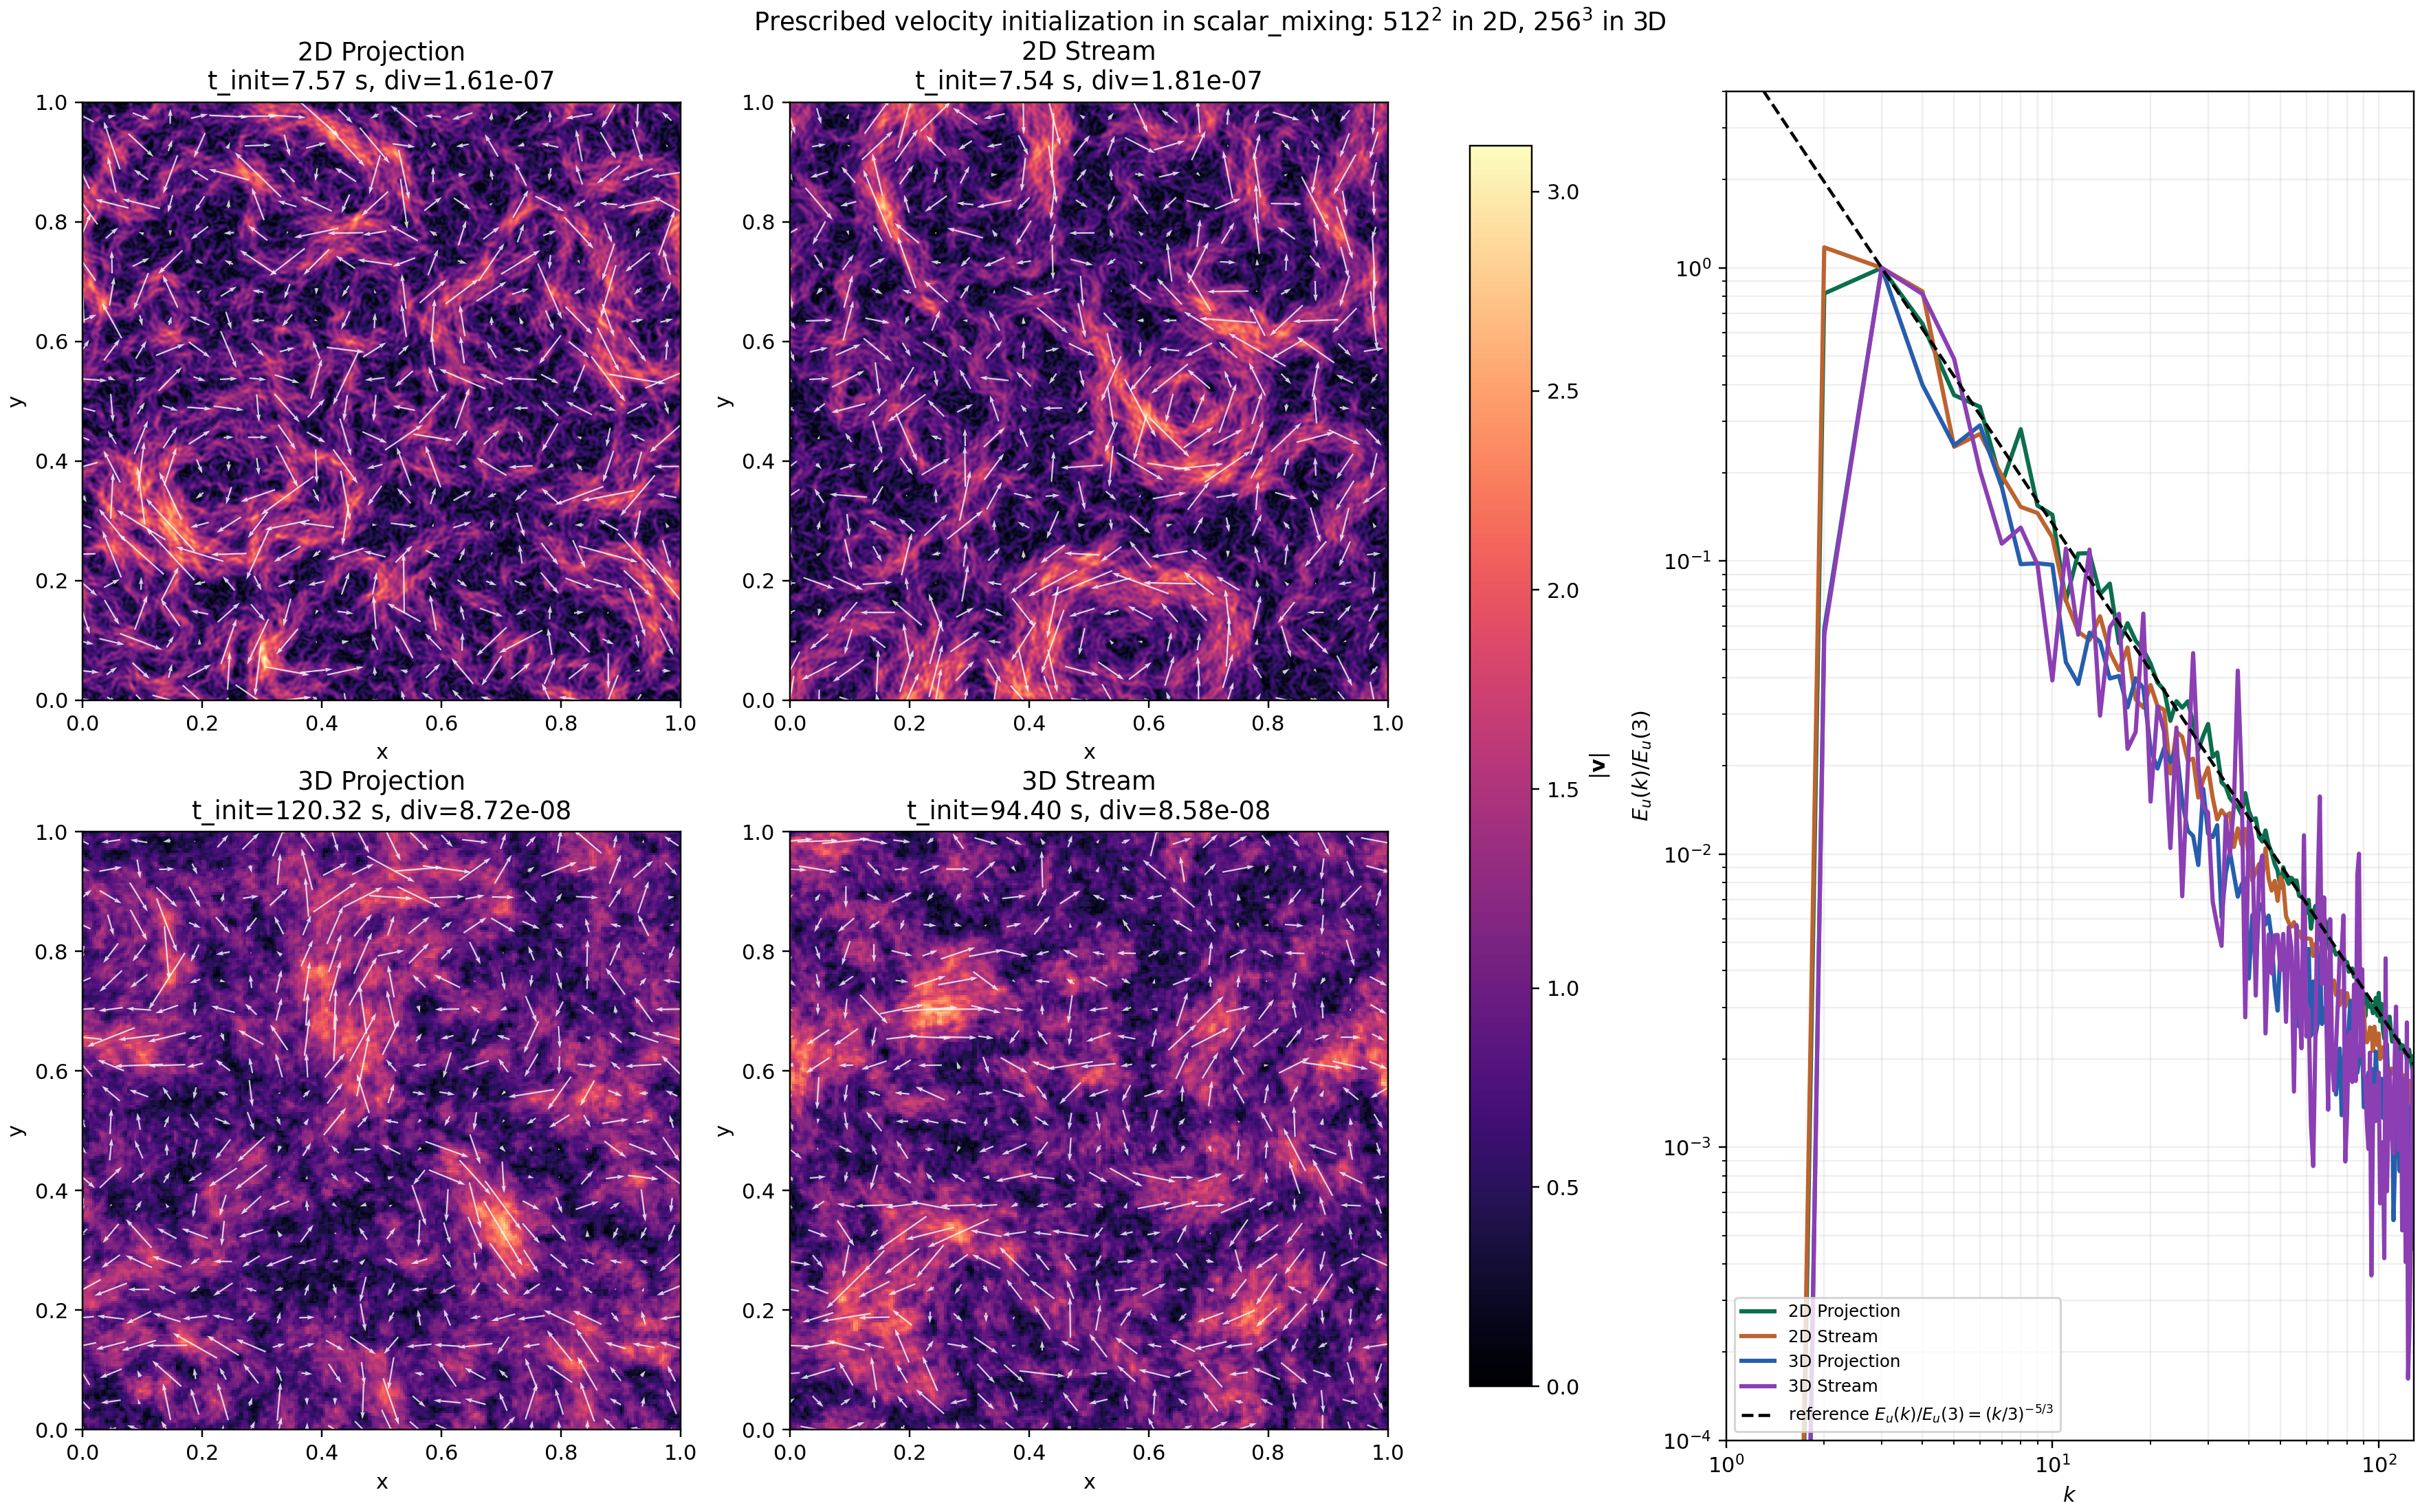
\includegraphics[width=\textwidth]{figures/scalar_mixing_velocity_methods/overview.png}
\caption{Overview of the four implemented velocity generators. The slice panels
show representative initialized speed fields for 2D projection, 2D stream, 3D
projection, and 3D Clebsch. The spectrum panel shows the corresponding
shape-normalized velocity spectra together with the target $k^{-5/3}$ law. The
titles report the measured initialization time and the spectral divergence
norm.}
\label{fig:overview}
\end{figure}

The method-specific figures clarify what the overview compresses. In 2D, projection and stream initialization produce different latent objects but comparable velocity spectra. The stream-function field is smoother than the velocity because $\psi$ carries the extra low-pass factor implied by Equation~(\ref{eq:psi-law}).

\begin{figure}[t]
\centering
\includegraphics[width=\textwidth]{figures/scalar_mixing_velocity_methods/methods_2d.png}
\caption{Two-dimensional generator diagnostics. Projection mode is shown through speed, vorticity, and velocity spectrum. Stream mode is shown through speed, latent stream function $\psi$, and the corresponding velocity and stream-function spectra. The target velocity spectrum is the same in both cases, but the latent field is steeper in stream mode because the velocity is obtained by differentiating $\psi$.}
\label{fig:methods-2d}
\end{figure}

In 3D the distinction is stronger. Projection mode is still a linear spectral
construction. Clebsch mode introduces two latent potentials whose retained shell
spectra are prescribed explicitly from the user-selected $\alpha$. The latent
spectra are therefore easy to interpret, while the velocity spectrum remains an
approximate consequence of the quadratic Clebsch product.

\begin{figure}[t]
\centering
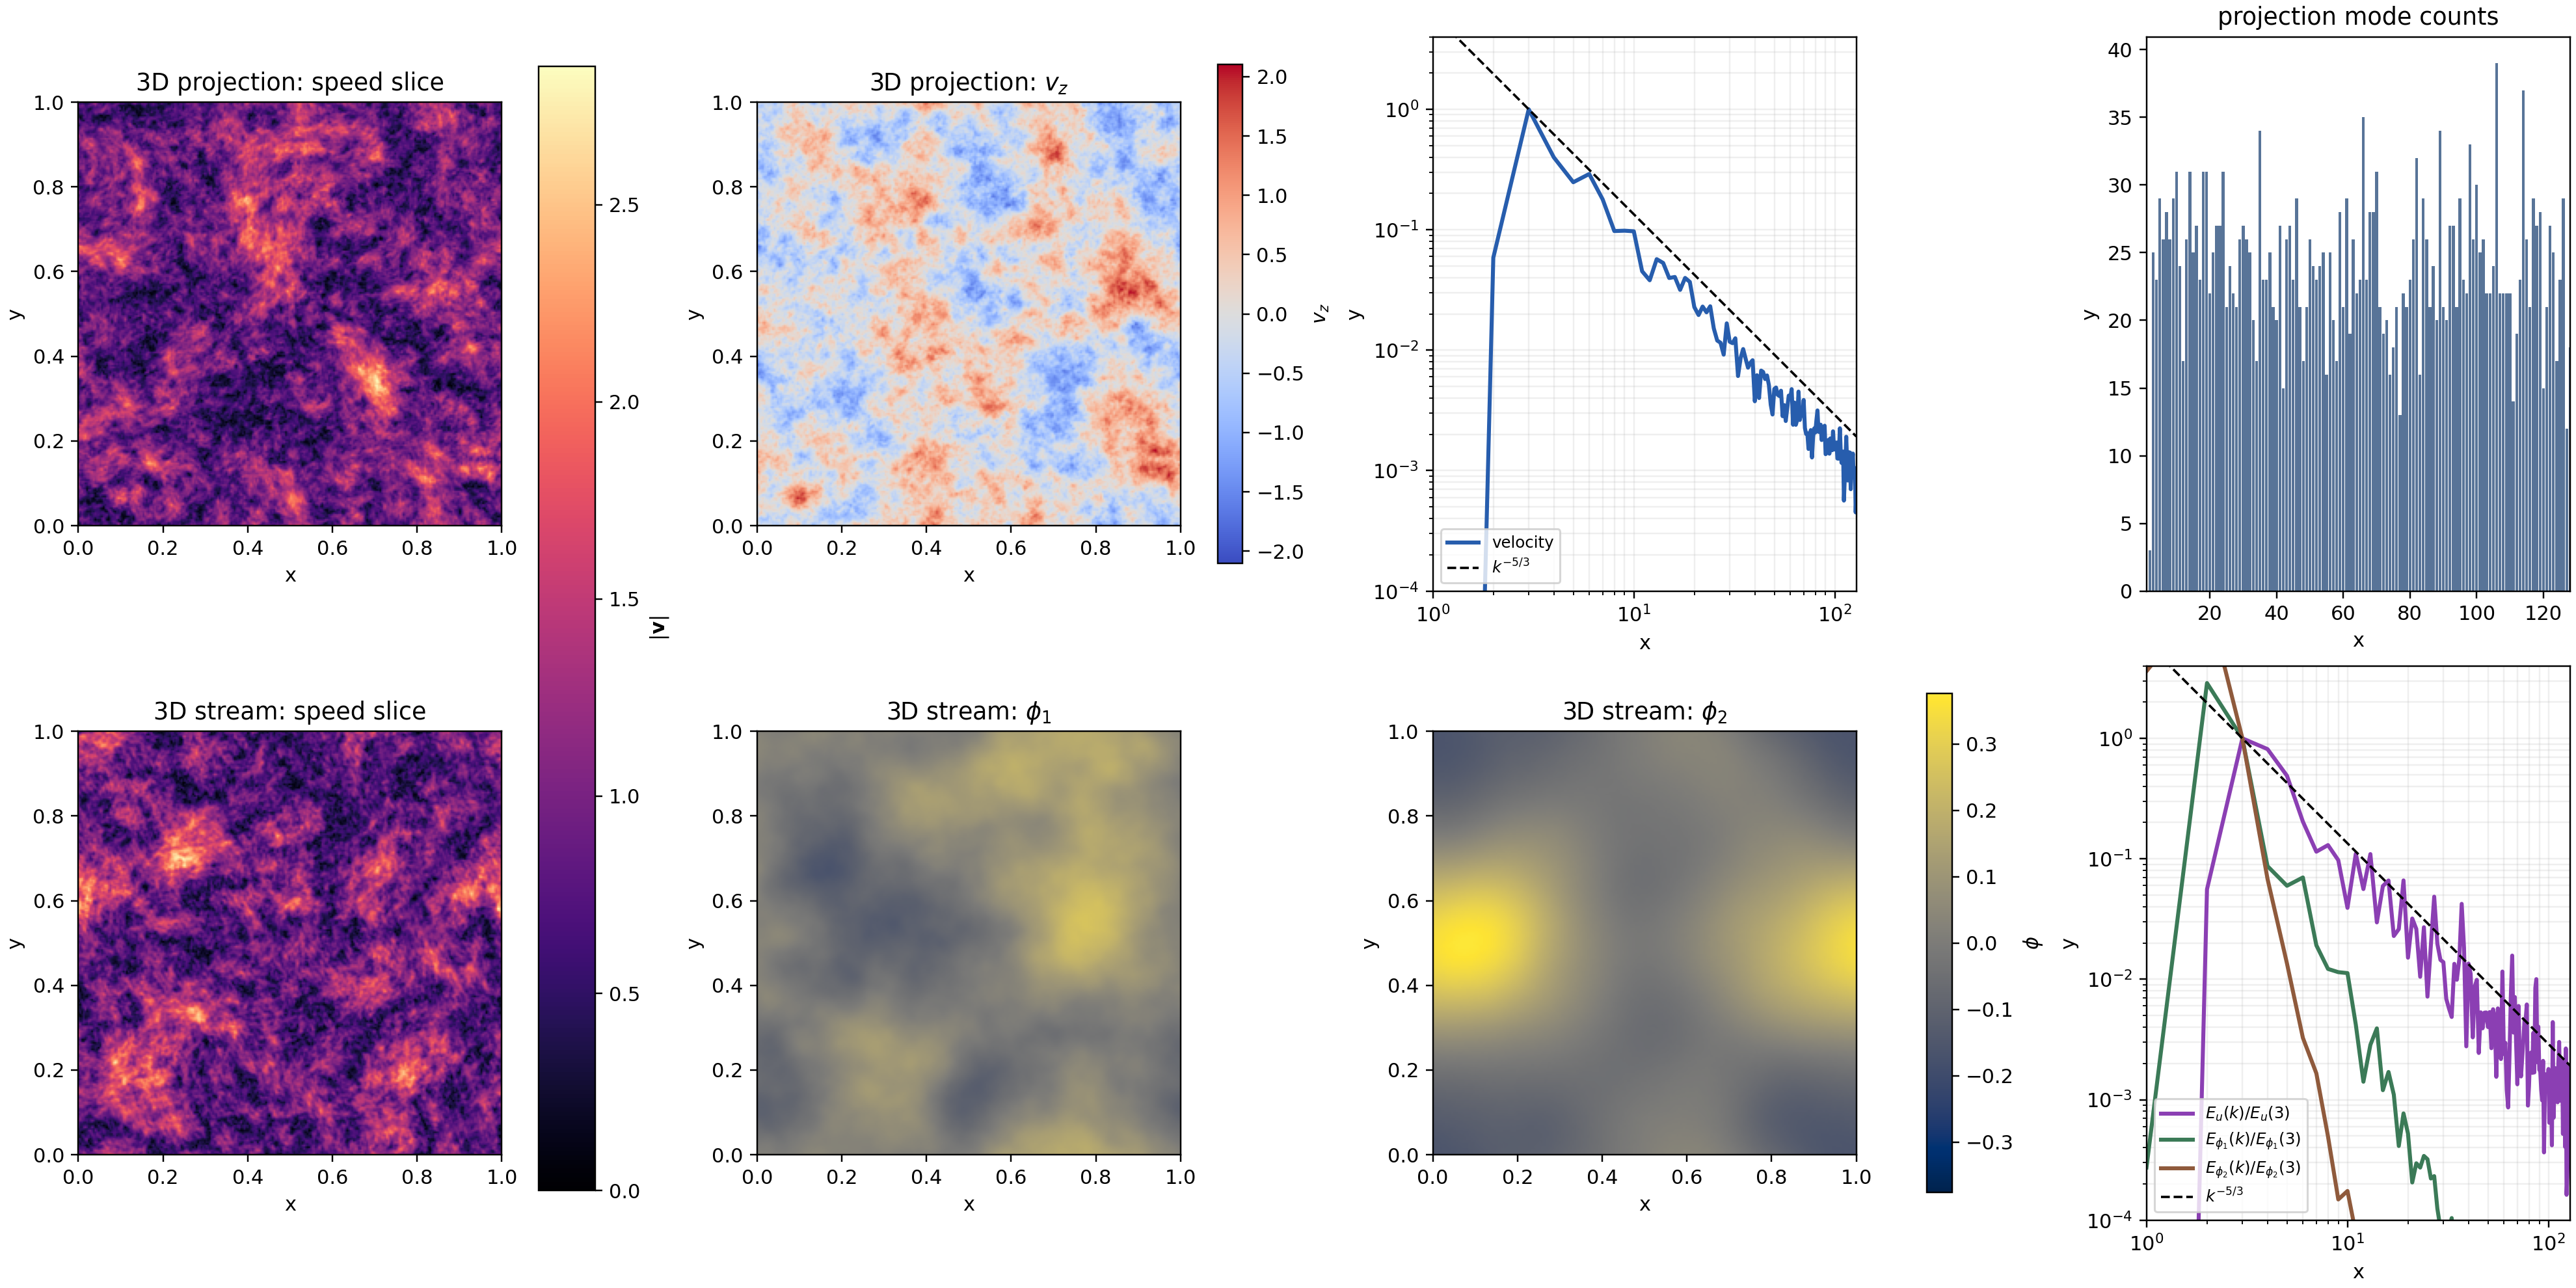
\includegraphics[width=\textwidth]{figures/scalar_mixing_velocity_methods/methods_3d.png}
\caption{Three-dimensional generator diagnostics. Projection mode is shown
through a midplane speed slice, a representative velocity-component slice, the
velocity spectrum, and the retained mode counts. Clebsch mode is shown through
a midplane speed slice, the latent potentials $\phi_1$ and $\phi_2$, and the
associated scalar and velocity spectra.}
\label{fig:methods-3d}
\end{figure}

The detailed 3D Clebsch diagnostics are especially important because this
remains the least direct mapping from user inputs to a realized velocity field.
The single-seed figure now emphasizes the quantities that actually exist in the
current implementation: the latent midplane slices, the exact retained scalar
shell laws, and the retained-versus-FFT velocity spectra for one representative
production-seed run.

\begin{figure}[t]
\centering
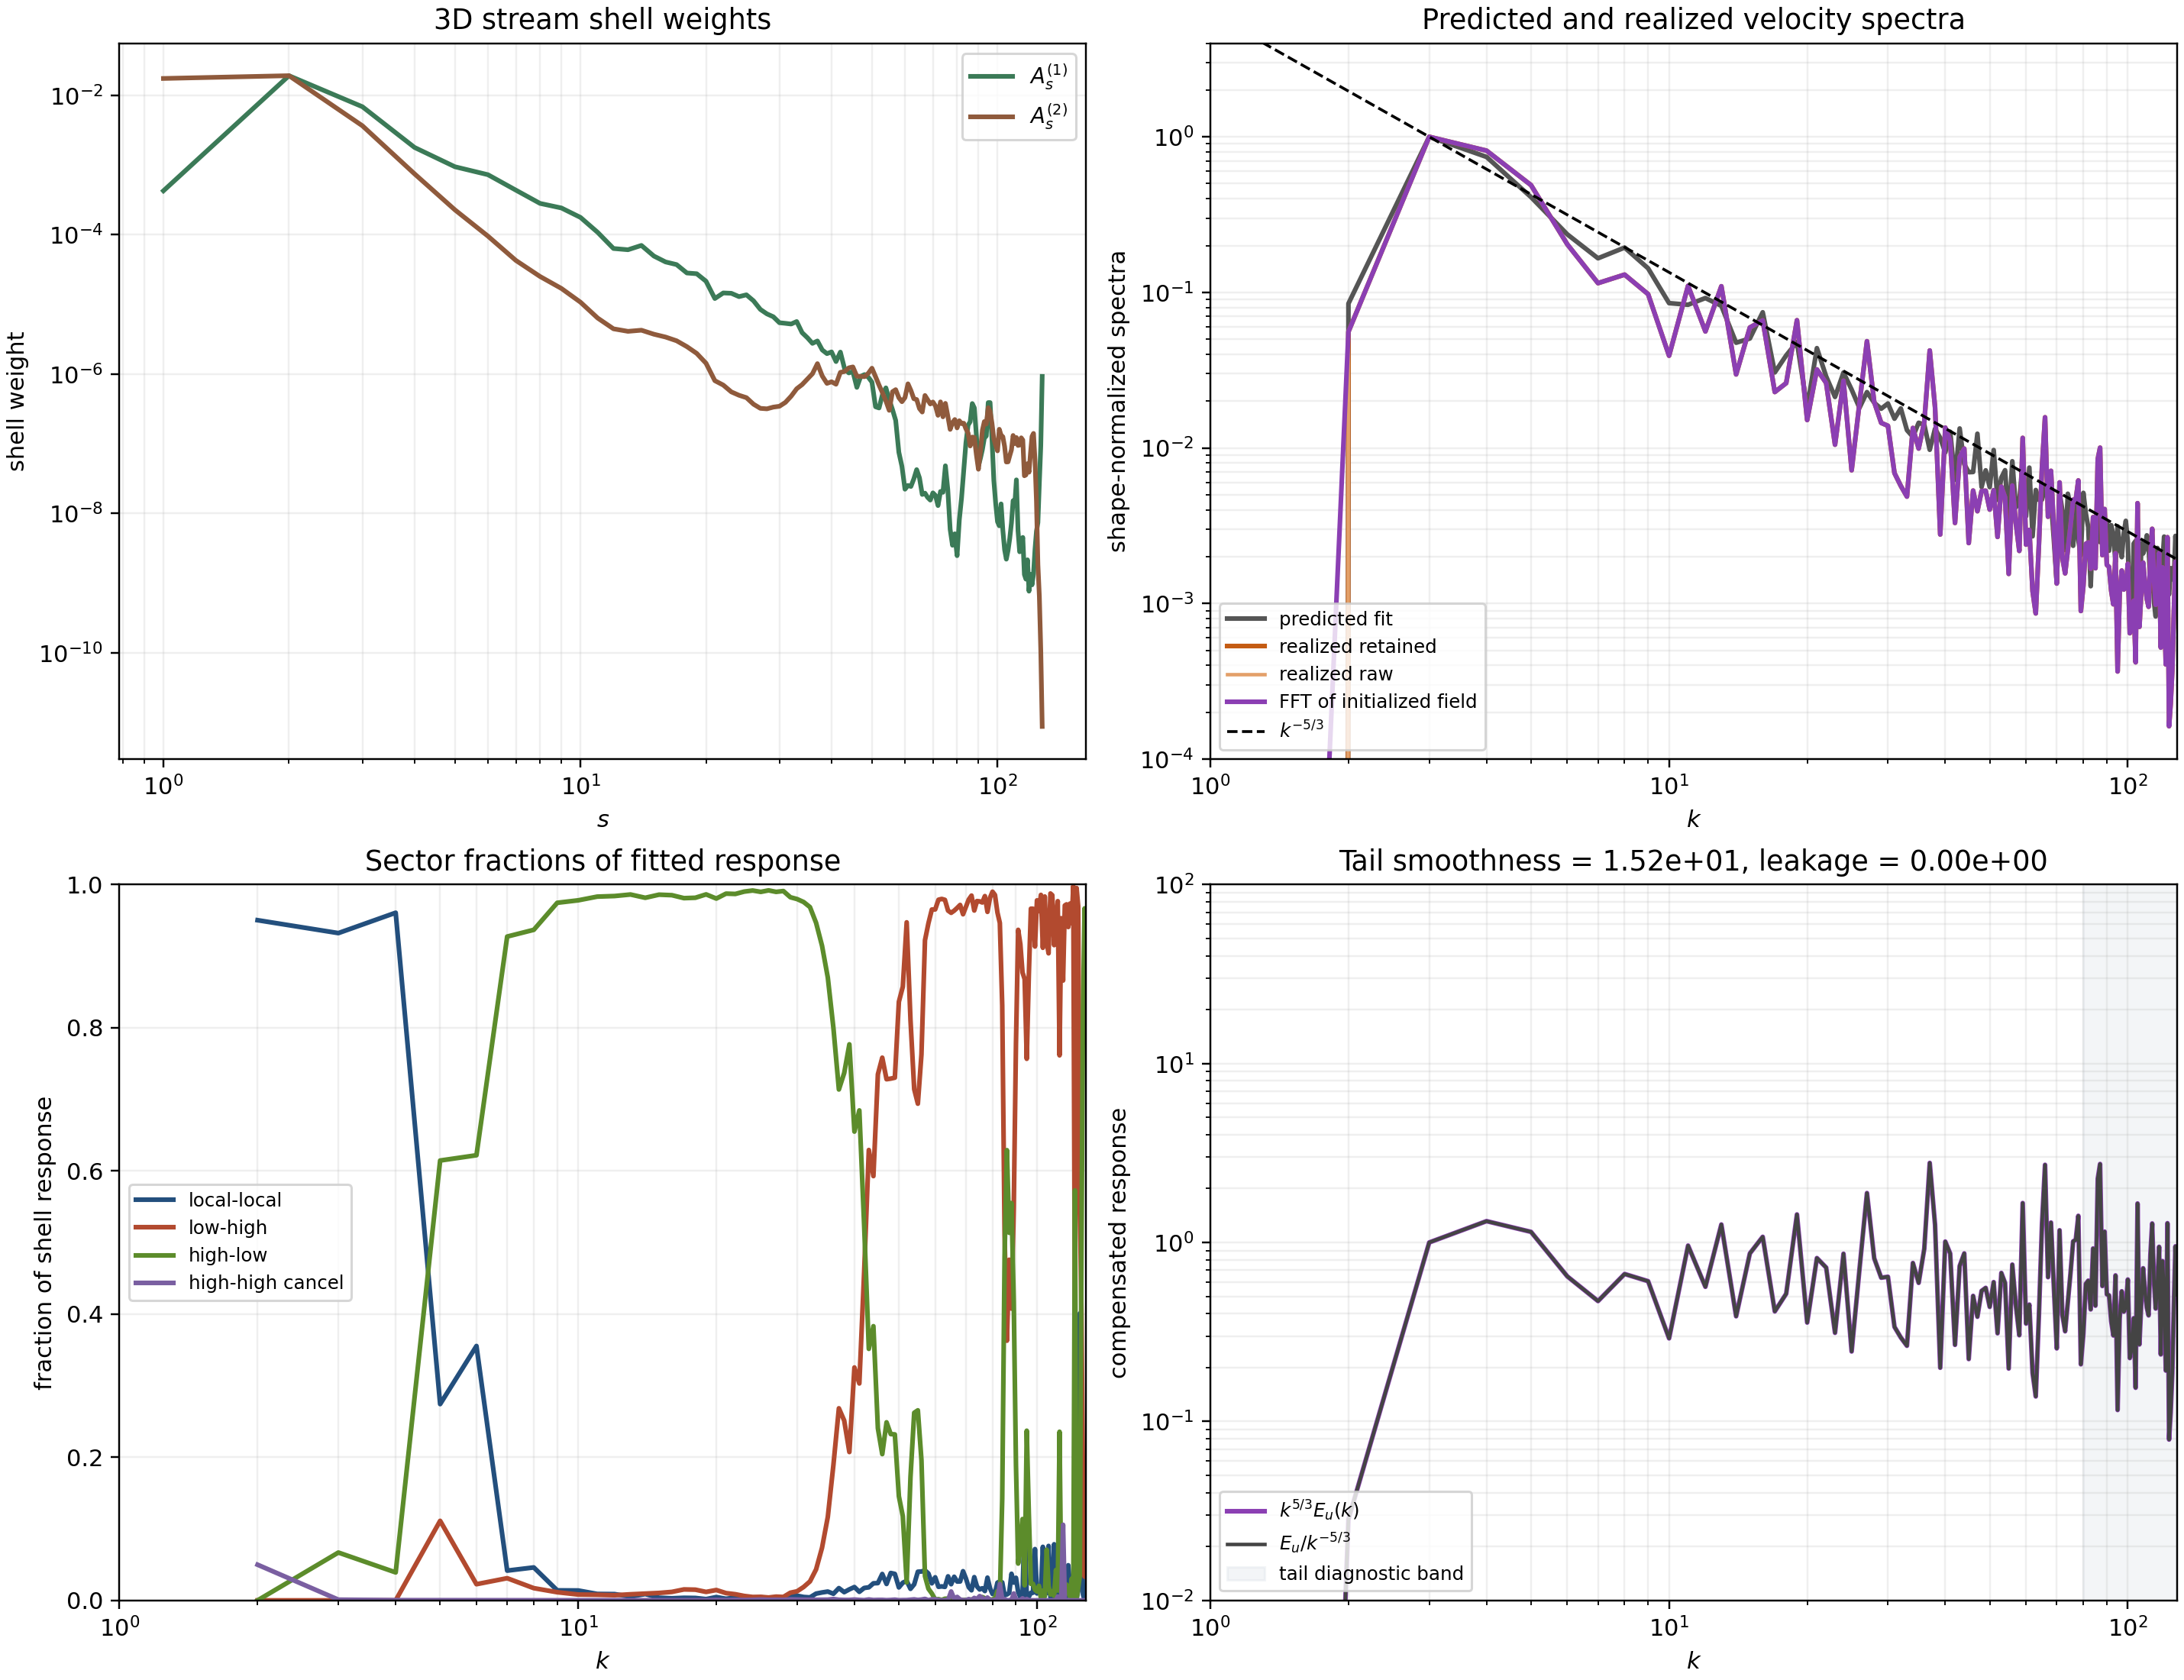
\includegraphics[width=\textwidth]{figures/scalar_mixing_velocity_methods/stream3d_realization.png}
\caption{Representative single-seed diagnostics of the 3D Clebsch
construction. The top row shows the two latent potentials on the midplane. The
lower-left panel shows their exact retained-shell spectra, and the lower-right
panel compares the retained Clebsch velocity spectrum with the FFT of the
initialized field. The important point is that the latent scalar spectra are
now explicit and exact on the retained shell band, while the realized velocity
spectrum remains a controlled approximation to the requested slope.}
\label{fig:clebsch3d-realization}
\end{figure}

Because the 3D Clebsch construction is stochastic, one representative
realization is not sufficient on its own. Figure~\ref{fig:clebsch3d-seed-audit}
summarizes the dedicated multi-seed audit. The upper panel overlays the
retained Clebsch spectra across seeds and audit cases, while the lower panel
tracks the mean retained slope and leakage. This is the scale-validation
counterpart to Figure~\ref{fig:clebsch3d-realization}.

\begin{figure}[t]
\centering
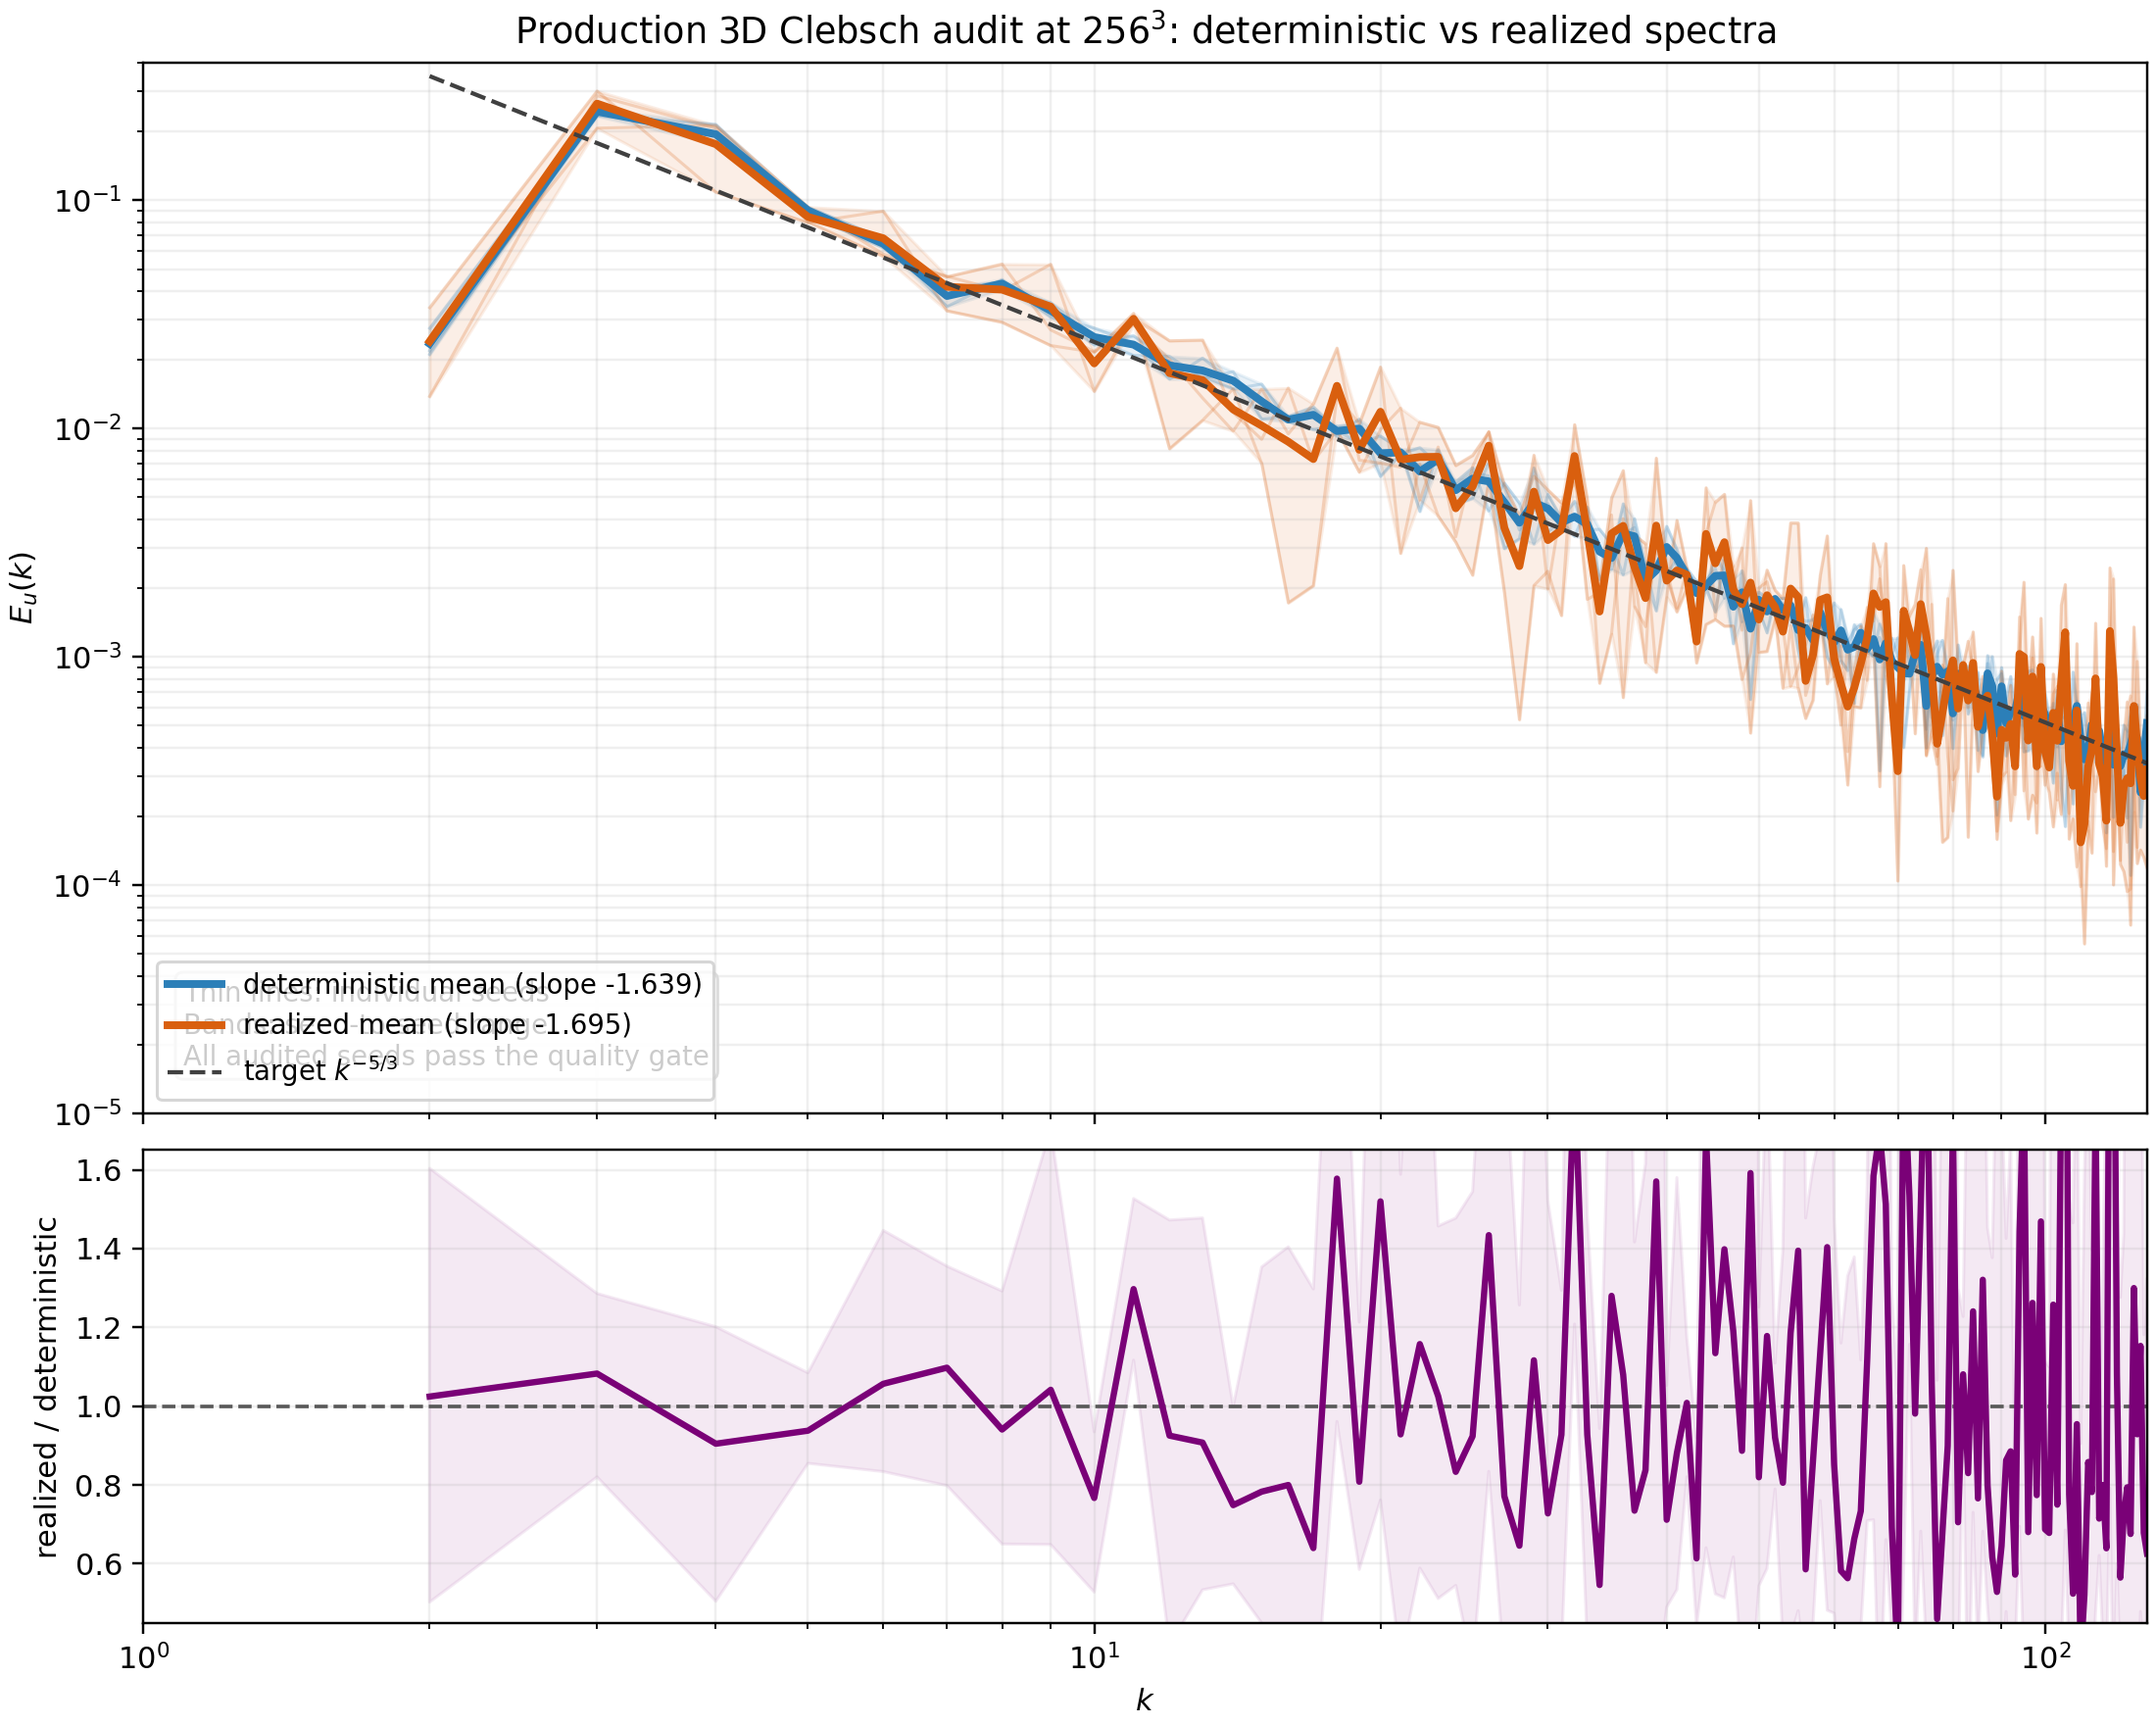
\includegraphics[width=\textwidth]{figures/scalar_mixing_velocity_methods/stream3d_production_audit.png}
\caption{Multi-seed audit of the 3D Clebsch construction. The upper panel shows
retained velocity spectra across seeds and audit cases, with bold curves for
the case means. The lower panel summarizes the mean retained slope magnitude
and leakage. This makes the retained-mode variability explicit without relying
on the deleted shell-fit or quality-gate machinery.}
\label{fig:clebsch3d-seed-audit}
\end{figure}

Taken together, the representative figures and the multi-seed audit justify the
velocity initialization as a standalone piece of the scalar-mixing problem. The
field that the scalar sees is divergence-free, has the requested band and rms
normalization, and follows the intended velocity slope to useful accuracy in
all four implemented modes.

\section{Scalar Advection--Diffusion and STS Tests}
Once the velocity field is prescribed, the scalar problem is only meaningful if the transport operator itself is the right one. In AthenaK that operator is \SO rather than \kin. The difference is essential. Under \SO the built-in hydrodynamic update is frozen, but the passive scalars still evolve conservatively using the hydro face mass flux and optional scalar diffusion. That diffusion can be advanced by the legacy explicit RK path or by the new RKL2 STS parabolic path. Under \kin the density and momentum equations are still advanced, so the hydro state is not actually frozen.

The scalar-side verification is handled by the dedicated \code{scalar\_mixing\_test} problem. In that test AthenaK advects and diffuses a passive-scalar blob in a uniform prescribed velocity field while the hydro background remains fixed. The analytic reference solution is computed from the exact AthenaK cell-centered initial condition by evolving its Fourier coefficients under uniform advection plus diffusion. This ensures that the comparison is aligned with the discrete initialization actually used by the code.

The STS version of this benchmark is enabled with two input switches:
\begin{center}
\code{time/sts\_integrator=rkl2},\qquad
\code{hydro/scalar\_diffusivity\_integrator=sts}.
\end{center}
The scalar diffusive flux is then omitted from the ordinary RK fluxes and advanced in parabolic pre- and post-sweeps, each over half of the cycle timestep. The explicit path remains the default when \code{scalar\_diffusivity\_integrator} is omitted. For the top-hat analytic tests the STS inputs set \code{hydro/sfloor=-1.0e100}, which disables scalar clipping so that the mass diagnostic measures the conservative update rather than mass added by clipping small undershoots near the diffusing discontinuity.

Figure~\ref{fig:blob-slices} shows the time evolution in 2D and 3D. In both cases the scalar advects and diffuses as expected while the background velocity remains uniform and the hydro state stays fixed. This establishes the correct frozen-hydrodynamic transport semantics before the more complicated turbulent initializations are used.

\begin{figure}[t]
\centering
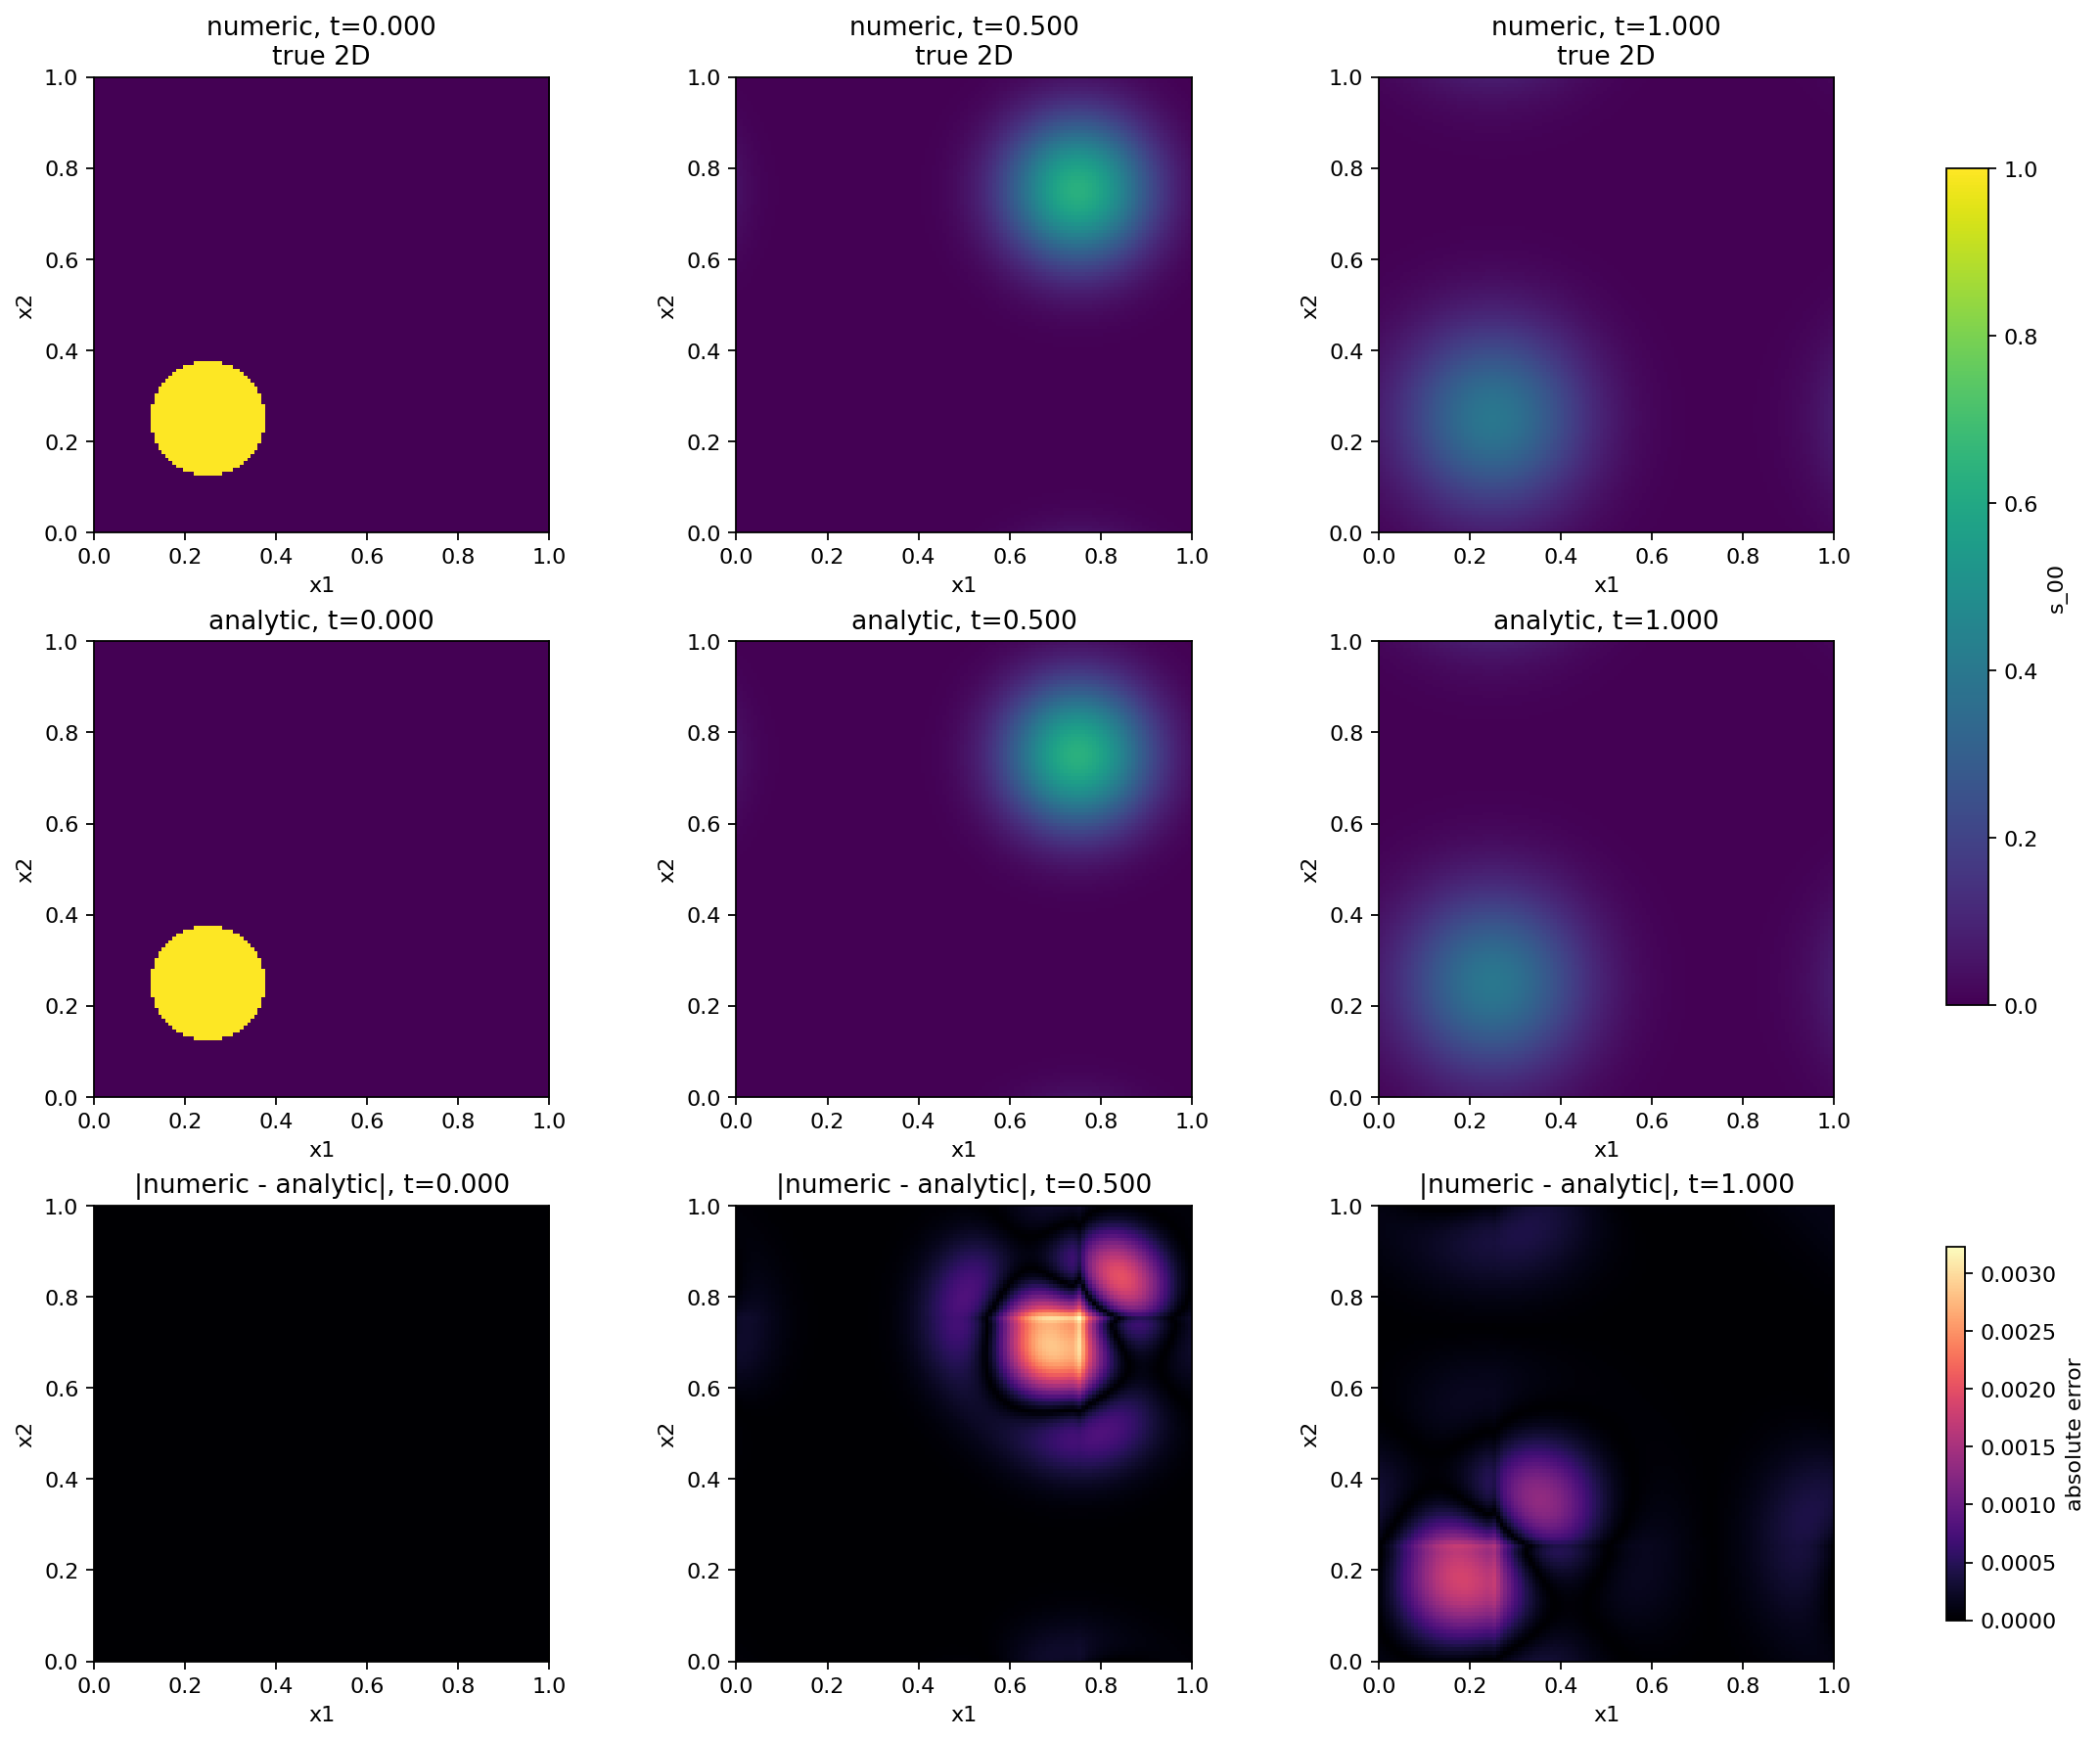
\includegraphics[width=0.49\textwidth]{figures/scalar_mixing_test/scalar_mixing_blob_diffusion_2d_time_slices.png}\hfill
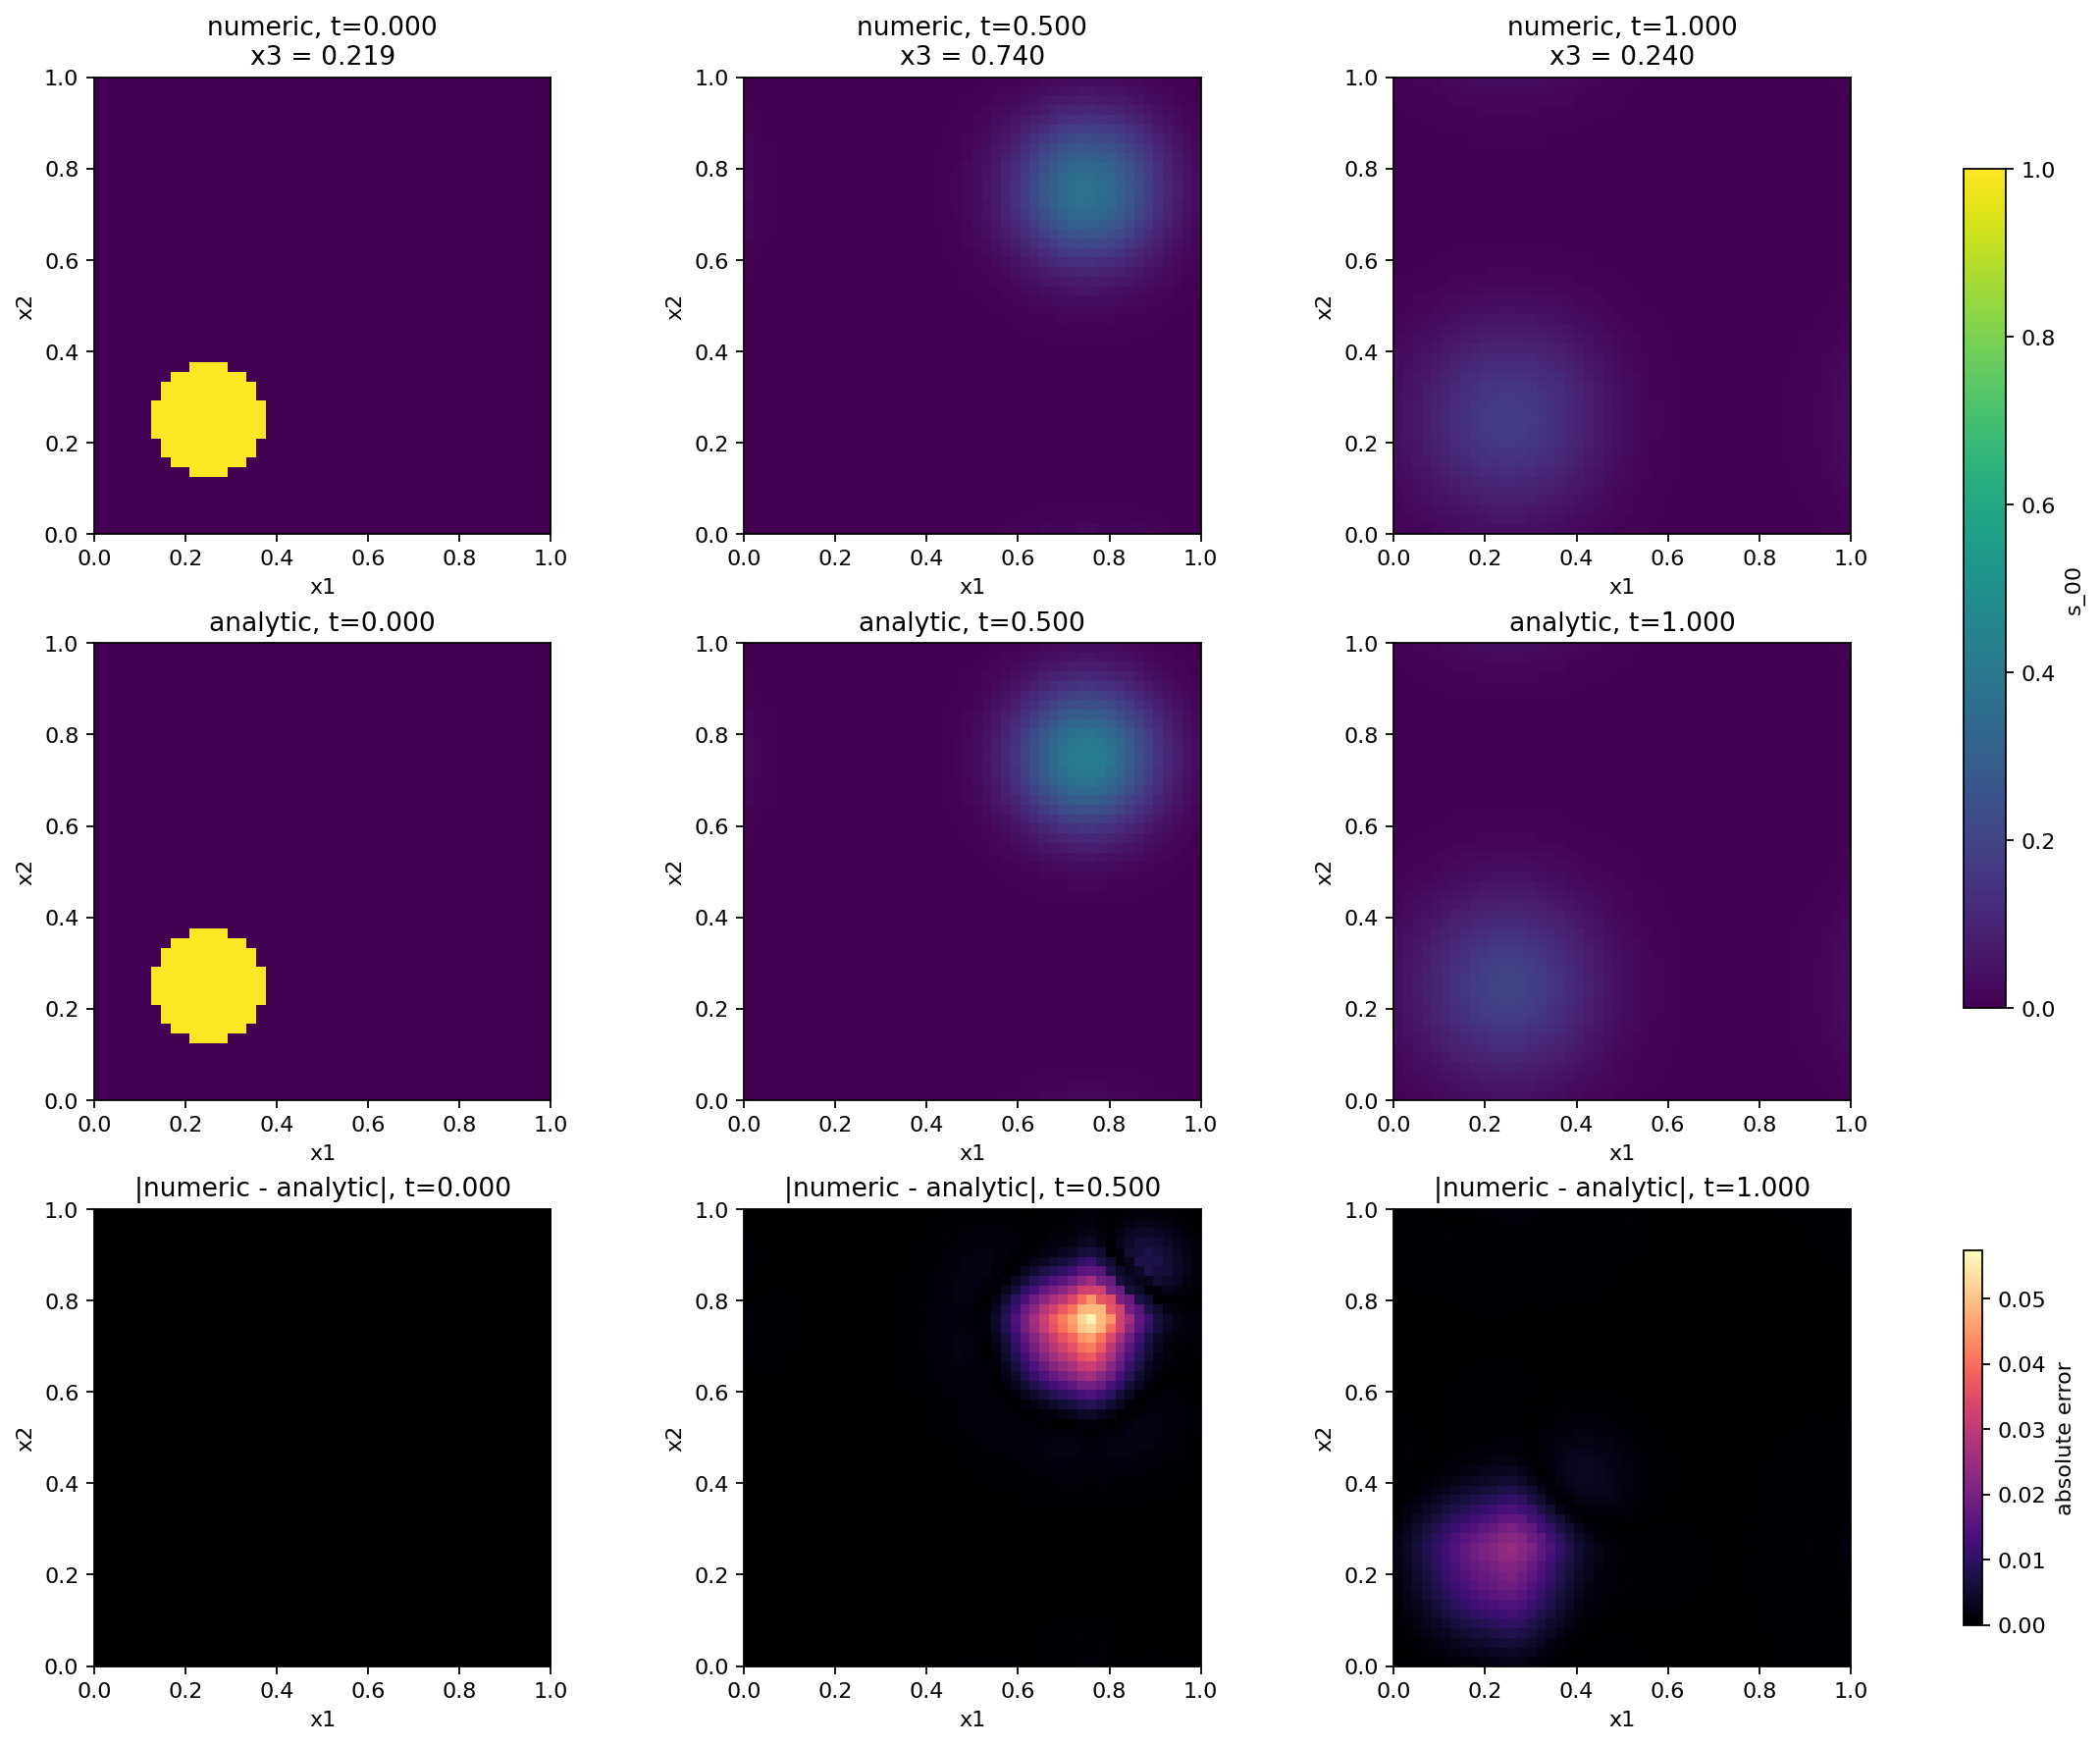
\includegraphics[width=0.49\textwidth]{figures/scalar_mixing_test/scalar_mixing_blob_diffusion_3d_time_slices.png}
\caption{Time-slice verification of the frozen scalar advection--diffusion operator in 2D and 3D. The scalar blob is transported by a prescribed uniform flow and diffuses as expected while the hydro background remains fixed.}
\label{fig:blob-slices}
\end{figure}

The convergence plots show that this agreement is not merely visual. In the calibrated diffusive families at $t=1$ and $\kappa=1/128$, the 2D errors decrease cleanly with resolution, with the $L^1$ error dropping from $9.27\times10^{-4}$ at $64^2$ to $1.96\times10^{-4}$ at $128^2$ and $4.65\times10^{-5}$ at $256^2$. The stable 3D family also improves systematically, with the $L^1$ error decreasing from $6.17\times10^{-4}$ at $48^3$ to $1.93\times10^{-4}$ at $64^3$ and $1.18\times10^{-4}$ at $80^3$. In addition, pure-advection smoke tests at CFL $0.2$ retain mass to roughly $10^{-10}$ relative accuracy in both 2D and 3D.

The STS regression uses the same final-time analytic checks rather than a separate looser standard. Table~\ref{tab:sts-blob-results-master} compares the explicit and STS paths on the shipped 2D and 3D diffusive blob inputs. Both STS runs pass the same field-error, mass, centroid, width, and velocity-uniformity thresholds as the explicit runs. The cycle counts also show the practical reason for making STS a primary scalar-diffusion mode: at these resolutions the 2D run drops from 1281 cycles to 320, and the 3D run drops from 271 cycles to 121.

\begin{table}[t]
\centering
\small
\caption{Analytic scalar advection--diffusion test results at $t=1$ and $\kappa=1/128$. All cases use \SO and the same Fourier-evolved reference solution.}
\begin{tabular}{llrrrr}
\hline
Case & Integrator & Cycles & $L^1$ & $L^\infty$ & Mass rel. \\
\hline
2D $128^2$ & explicit RK & 1281 & $1.962\times10^{-4}$ & $1.851\times10^{-3}$ & $3.016\times10^{-10}$ \\
2D $128^2$ & RKL2 STS & 320 & $2.778\times10^{-4}$ & $2.650\times10^{-3}$ & $1.633\times10^{-10}$ \\
3D $48^3$ & explicit RK & 271 & $6.168\times10^{-4}$ & $2.451\times10^{-2}$ & $1.766\times10^{-10}$ \\
3D $48^3$ & RKL2 STS & 121 & $4.931\times10^{-4}$ & $1.597\times10^{-2}$ & $1.081\times10^{-9}$ \\
\hline
\end{tabular}
\label{tab:sts-blob-results-master}
\end{table}

\begin{figure}[t]
\centering
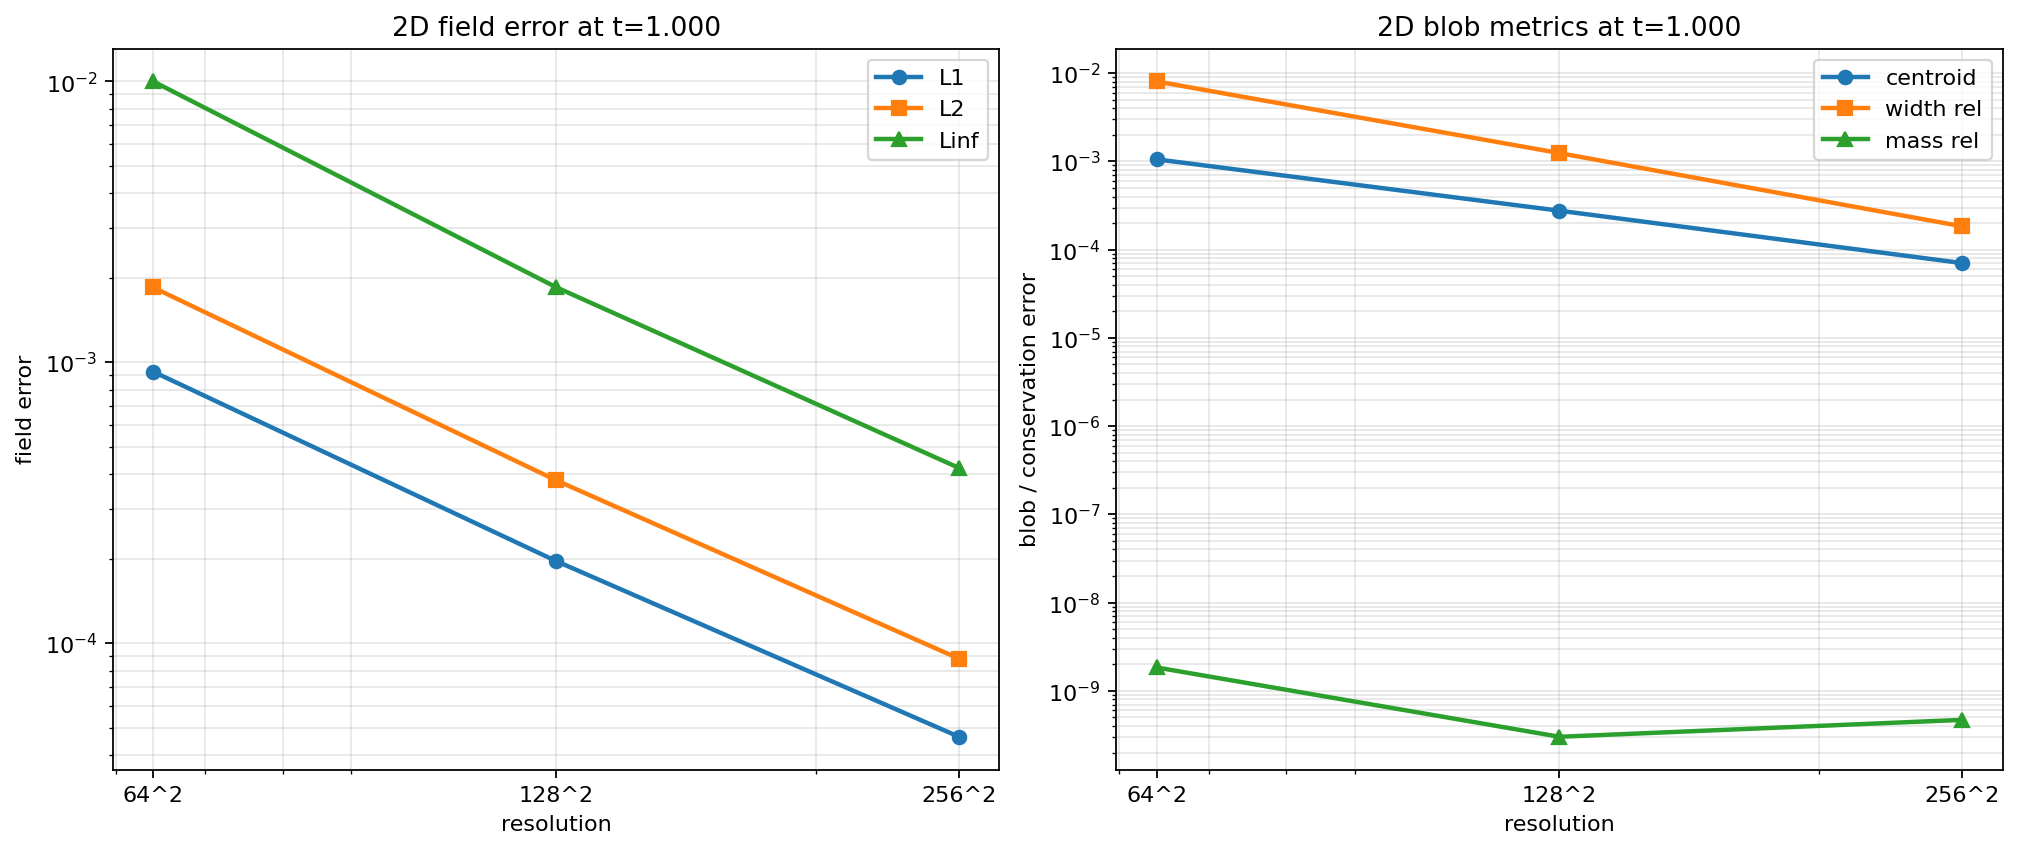
\includegraphics[width=0.49\textwidth]{figures/scalar_mixing_test/scalar_mixing_test_convergence_2d_t1p0.png}\hfill
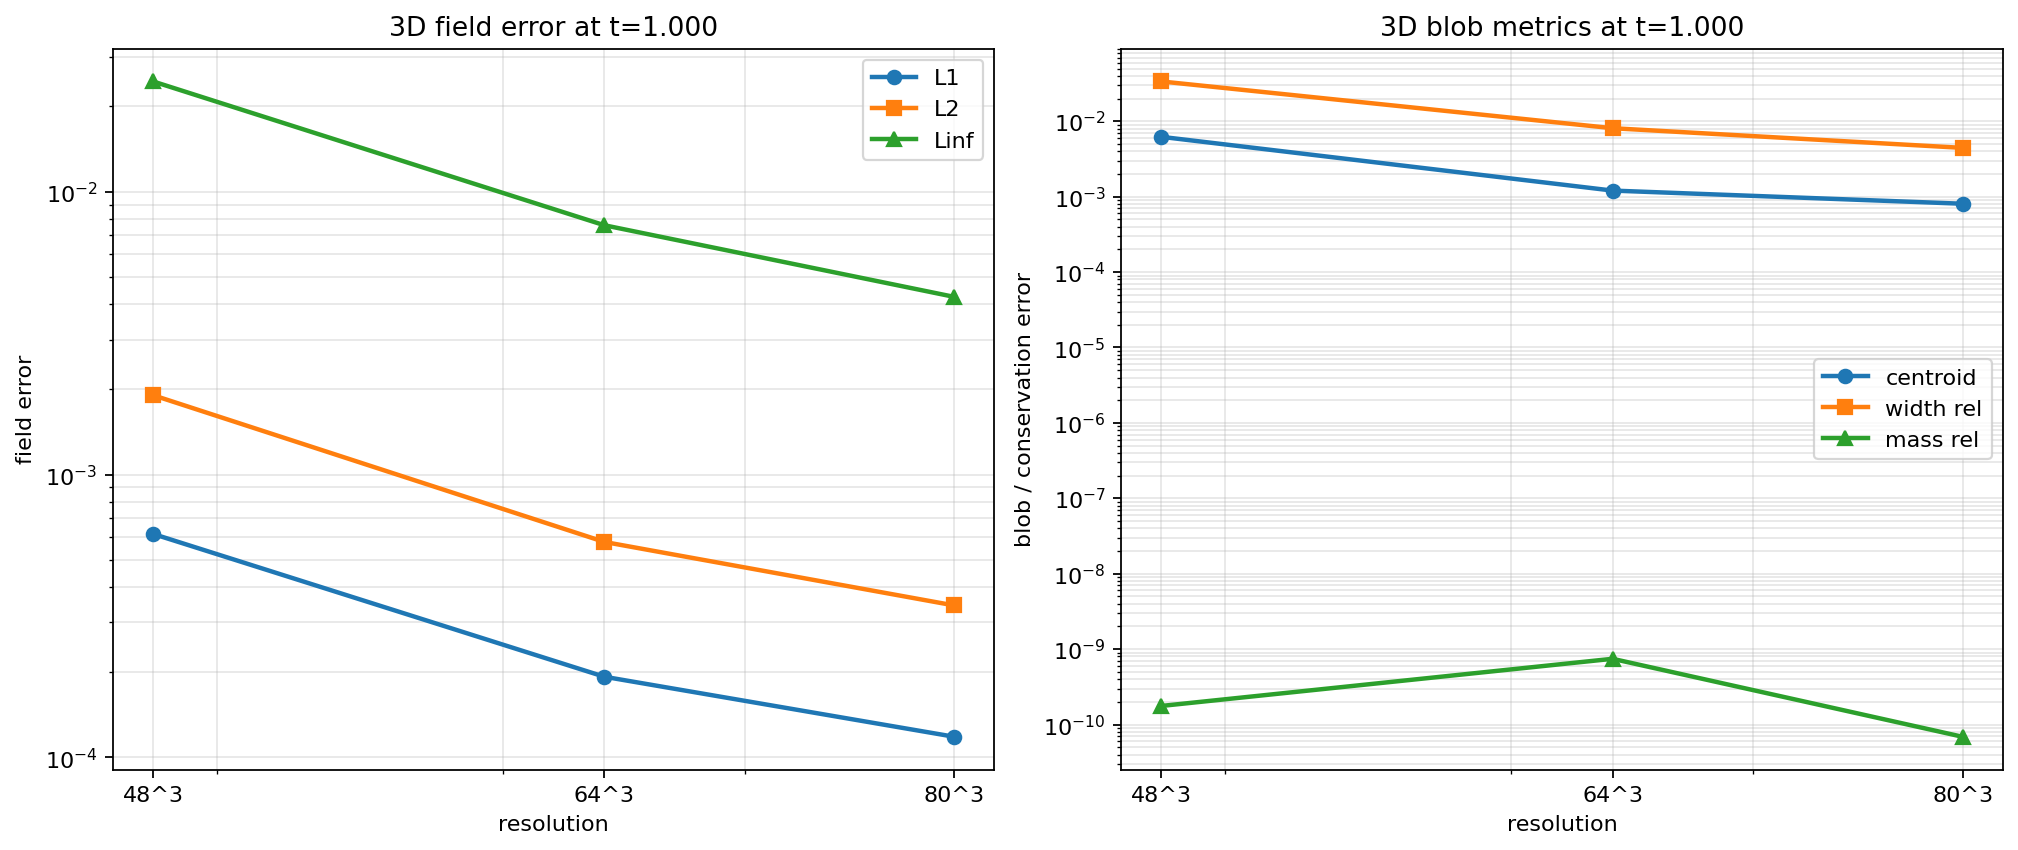
\includegraphics[width=0.49\textwidth]{figures/scalar_mixing_test/scalar_mixing_test_convergence_3d_t1p0.png}
\caption{Resolution/error convergence for the scalar advection--diffusion verification problem at $t=1$. The 2D sequence shows a clean reduction of norm, centroid, and width errors with refinement. The 3D sequence is somewhat noisier and requires avoiding the most underresolved meshes, but the stable reference family still converges systematically toward the analytic solution.}
\label{fig:blob-convergence}
\end{figure}

These tests close the numerical loop. The velocity generator is validated independently of the scalar solver, and the scalar solver is validated independently of the turbulent velocity generator. Together they define the full prescribed-velocity scalar-mixing problem actually executed by AthenaK.

\section{Conclusions}
The merged picture is straightforward.

First, the scientific question should be stated in finite-time form. The relevant observable is the integrated scalar dissipation $\chi_D(T)$ over one to a few advective times, not an asymptotic late-time limit in which the scalar simply decays to its mean.

Second, the roughness dictionary must be handled carefully. The spectral slope $\zeta$ is the direct numerical input. The relation $\alpha=(\zeta-1)/2$ is a classical H\"older statement only when $1<\zeta<3$; for $\alpha\le 0$ it becomes a negative regularity index and must be interpreted distributionally.

Third, the velocity setup now has a coherent four-mode structure. Projection mode is the cleanest path when direct control of the initialized velocity spectrum is the main goal. Stream mode should be used when the latent scalar potential is physically meaningful. In 2D that latent object is the stream function $\psi$. In 3D it is the pair of Clebsch potentials $\phi_1$ and $\phi_2$, whose shell weights must be fitted because the velocity depends on them quadratically.

Fourth, the velocity generator and scalar transport operator have now both been tested in the form actually used by the code. The velocity campaign verifies spectral slope, divergence control, and latent-field diagnostics. The scalar verification problem confirms that \SO defines the correct frozen-hydrodynamic transport operator and that the scalar solution converges toward the analytic advection--diffusion reference. The same analytic benchmark now also confirms that RKL2 STS is a conservative and accurate primary path for scalar diffusion when the parabolic timestep would otherwise dominate the cost.

This is the sense in which the present document functions as a master note. It starts from the general scalar-mixing question, translates the roughness parameters, documents the velocity generators, and ends with the tests that justify using the implementation for actual scalar-advection studies.

\end{document}
